\newpage
\section{Proxy Pattern}

In proxy pattern, a class represents functionality of another class. This type of design pattern comes under structural pattern.

In proxy pattern, we create object having original object to interface its functionality to outer world.

\subsection{Implementation}

We are going to create an Image interface and concrete classes implementing the Image interface. ProxyImage is a a proxy class to reduce memory footprint of RealImage object loading.

ProxyPatternDemo, our demo class, will use ProxyImage to get an Image object to load and display as it needs.

\subsection{Class Diagram}

\begin{figure}[h]
\centering
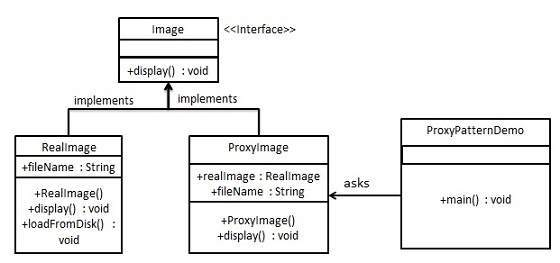
\includegraphics[scale=0.7]{proxy}
\caption{Class Diagram of Proxy Pattern}
\end{figure}

\newpage
\subsection{Source Code (Java)}

\subsubsection{Image Interface}

\begin{minted}{java}
public interface Image {
   void display();
}
\end{minted}

\subsubsection{RealImage Class}

\begin{minted}{java}
public class RealImage implements Image {

   private String fileName;

   public RealImage(String fileName){
      this.fileName = fileName;
      loadFromDisk(fileName);
   }

   @Override
   public void display() {
      System.out.println("Displaying " + fileName);
   }

   private void loadFromDisk(String fileName){
      System.out.println("Loading " + fileName);
   }
}
\end{minted}

\subsubsection{ProxyImage Class}

\begin{minted}{java}
public class ProxyImage implements Image{

   private RealImage realImage;
   private String fileName;

   public ProxyImage(String fileName){
      this.fileName = fileName;
   }

   @Override
   public void display() {
      if(realImage == null){
         realImage = new RealImage(fileName);
      }
      realImage.display();
   }
}
\end{minted}

\subsubsection{Driver Class}

\begin{minted}{java}
public class ProxyPatternDemo {
	
   public static void main(String[] args) {
      Image image = new ProxyImage("test_10mb.jpg");

      //image will be loaded from disk
      image.display(); 
      System.out.println("");
      
      //image will not be loaded from disk
      image.display(); 	
   }
}
\end{minted}

\subsection{Output}

\begin{minted}{text}
Loading test_10mb.jpg
Displaying test_10mb.jpg

Displaying test_10mb.jpg
\end{minted}
